% CSCI3753 - Operating Systems
% Spring 2012
% Programming Assignment 4
% By Andy Sayler (3/6/12)

\documentclass[12pt]{article}

\usepackage[text={6.5in, 9in}, centering]{geometry}
\usepackage{graphicx}
\usepackage{url}
\usepackage{listings}
\usepackage{hyperref}

\lstset{
  language={},
  morekeywords={for,end,run,if,else,endif,exit,endprog,goto},
  basicstyle=\footnotesize,
  numbers=left,
  numberstyle=\tiny,
  stepnumber=1,
  numbersep=5pt,
  showspaces=false,
  showstringspaces=false,
  showtabs=false,
  tabsize=4,
  captionpos=b,
  breaklines=true,
  breakatwhitespace=false,
  frame=single,
  frameround=tttt
}

\hypersetup{
    colorlinks,
    citecolor=black,
    filecolor=black,
    linkcolor=black,
    urlcolor=black
}

\newenvironment{packed_enum}{
\begin{enumerate}
  \setlength{\itemsep}{1pt}
  \setlength{\parskip}{0pt}
  \setlength{\parsep}{0pt}
}{\end{enumerate}}

\newenvironment{packed_item}{
\begin{itemize}
  \setlength{\itemsep}{1pt}
  \setlength{\parskip}{0pt}
  \setlength{\parsep}{0pt}
}{\end{itemize}}

\newenvironment{packed_desc}{
\begin{description}
  \setlength{\itemsep}{1pt}
  \setlength{\parskip}{0pt}
  \setlength{\parsep}{0pt}
}{\end{description}}

\title{Programming Assignment 4:\\Virtual Memory Paging Strategies}
\author{
  CSCI 3753 - Operating Systems\\
  University of Colorado at Boulder\\
  Spring 2012\\
  By Andy Sayler and Junho Ahn and Richard Han\\
  Adopted from assignment by Dr. Alva Couch, Tufts University\cite{couch-a5}
}
\date{\emph{Due Date: Wednesday, April 18th, 2012 11:55pm}}

\begin{document}

\maketitle

\section{Assignment Introduction}

All modern operating systems use virtual memory and paging in order to
effectively utilize the computer's memory hierarchy. Paging is an
effective means of providing memory space protection to processes, of
enabling the system to utilize secondary storage for additional
memory space, and of avoiding the need to allocate memory sequentially
for each process.

We have studied how virtual memory systems are structured and how the MMU
converts virtual memory addresses to physical memory addresses by
means of a page table and a translation lookaside buffer (TLB). When a
page has a valid mapping from VM address to physical address, we say
the page is ``swapped in''. When no valid mapping is available, the page
is either invalid (a segmentation fault), or more likely, ``swapped
out''. When the MMU determines that a memory request requires access to
a page that is currently swapped out, it calls the operating system's
page-fault handler. This handler must swap-in the necessary page,
possibly evicting another page to secondary memory in the process.
It then retries the
offending memory access and hands control back to the MMU.

As you might imagine, how the OS chooses which page to evict when it
has reached the limit of available physical pages (sometime called
frames) can have a major
effect on the performance of the memory access on a given system.
In this assignment, we will look at various strategies for managing
the system page table and controlling when pages are paged in and when
they are paged out.

\section{Your Task}

The goal of this assignment is to implement a paging strategy that
maximizes the performance of the memory access in a
set of predefined programs. You will accomplish this task by using a
paging simulator that has already been created for you. Your job is to
write the paging strategy that the simulator utilizes (roughly
equivalent to the role the page fault handler plays in a real OS). Your
initial goal will be to create a Least Recently Used paging
implementation. You will then need to implement some form of predictive
page algorithm to increase the performance of your solution.
You will be graded
on the throughput of your solution (the ratio of time spent doing
useful work vs time spent waiting on the necessary paging to occur).

\subsection {The Simulator Environment}

The simulator has been provided for you. You have access to the source
code if you wish to review it (\texttt{simulator.c} and
\texttt{simulator.h}), but you
should not need to modify this code for the sake of this
assignment. You will be graded using the stock simulator, so any
enhancements to the simulator program made with the intention of
improving your performance will be for naught.

The simulator runs a random set of programs utilizing a limited
number of shared physical pages. Each process has a fixed number of
virtual pages, the process's virtual memory space,
that it might try to access. For the purpose of this
simulation, all memory access is due to the need to load program
code. Thus, the simulated program counter (PC) for each process
dictates which memory location that process currently requires access
to, and thus which virtual page must be swapped-in for the
process to successfully continue.

The values of the constants mentioned above
are available in the \texttt{simulator.h} file. For the purposes of
grading your assignment, the default values will be used:

\begin{packed_item}
\item 20 virtual pages per process (\texttt{MAXPROCPAGES})
\item 100 physical pages (frames) total (\texttt{PHYSICALPAGES})
\item 20 simultaneous processes competing for pages (\texttt{MAXPROCESSES})
\item 128 memory unit page size (\texttt{PAGESIZE})
\item 100 tick delay to swap a page in or out (\texttt{PAGEWAIT})
\end{packed_item}

As you can see, you are working in a very resource constrained
environment. You will have to deal with attempts to access up to 400
virtual pages (20 processes times 20 virtual pages per process),
but may only have, at most, 100 physical pages swapped in at any given
time.

In addition, swapping a page
in or out is an expensive operation, requiring 100 ticks to
complete. A tick is the minimum time measurement unit in the
simulator. Each instruction or step in the simulated programs requires 1
tick to complete. Thus, in the worst case where every instruction is a
page miss (requiring a swap-in), you will spend 100 ticks of paging
overhead for every 1 tick of useful work. If all physical pages are in
use, this turns into 200 ticks per page miss since you must also
spend 100 ticks swapping a page out in order to make room for the
required page to be swapped in. This leads to an ``overhead to
useful work'' ratio of 200 to 1: very, very, poor performance. Your
goal is to implement a system that does much better than this worst case
scenario.

\subsection {The Simulator Interface}

The simulator exports three functions through which you will interact
with it. The first function is called \texttt{pageit}. This is the
core paging function. It is roughly equivalent to the page-fault handler in
your operating system. The simulator calls \texttt{pageit} anytime
something interesting happens (memory access, page fault, process
completion, etc). It passes the function a page map for each process,
as well as the current value of the program counter for each
process. See \texttt{simulator.h} for details. You will
implement your paging strategy in the body of this function.

The \texttt{pageit} function is passed an array of \texttt{pentry}
structs, one per process. This struct contains a copy of all of the
necessary memory information that the simulator maintains for each
process. You will need the information contained in this struct to make
intelligent paging decisions. It is the simulator's job to maintain
this information. You should just read it as necessary. The struct
contains:

\begin{packed_desc}
\item[\texttt{long active}] \hfill \\
  A flag indicating whether or not the
  process has completed. \texttt{1} if running, \texttt{0} if exited.
\item[\texttt{long pc}] \hfill \\
  The value of the program counter for the
  process. The current page can be calculated as $page = pc / PAGESIZE$.
\item[\texttt{long npages}] \hfill \\
  The number of pages in the processes
  memory space. If the process is active (running), this will be equal
  to MAXPROCPAGES. If the process has exited, this will be 0.
\item[\texttt{long pages[MAXPROCPAGES]}] \hfill \\
  A bitmap array representing the
  page map for a given process. If \texttt{pages[X]} is
  \texttt{0}, page X is swapped out, swapping out, or swapping in.
  If \texttt{pages[X]} is \texttt{1}, page X is currently swapped in.
\end{packed_desc}

The simulator also exports a function called \texttt{pagein} and a
function called \texttt{pageout}. These functions request that a
specific page for a specific process be swapped in or swapped out,
respectively. You will use these function to control the allocation of
virtual and physical pages when writing your paging strategy. Each of
these functions returns \texttt{1} if they succeed in \emph{starting} a
paging operation, if the requested paging operation is \emph{already in
  progress}, or if the \emph{requested state already exists}.
100 ticks after requesting a paging operation, the
operation will complete. When calling \texttt{pagein}, the page maps passed
to \texttt{pageit}
will reflect the new state of the simulator after the request
completes 100 ticks later. When calling \texttt{pageout}, the page maps passed
to \texttt{pageit}
will reflect the new state of the simulator in the first call to
\texttt{pageit} after the request is made.
In short, a page is recognized as swapped out as soon as a
\texttt{pageout} request is made, but is not recognized as swapped in
until after a \texttt{pagein} request completes.
These functions return
\texttt{0} if the paging request can not be processed (due to
exceeding the limit of physical pages or because another paging
operation is currently in process on the requested page) or if the
request is invalid (paging operation requests non-existent page,
etc). See Figure \ref{fig:pagestate} for more details on the behavior
of \texttt{pagein} and \texttt{pageout}.

\begin{figure}[htbp]
  \begin{center}
    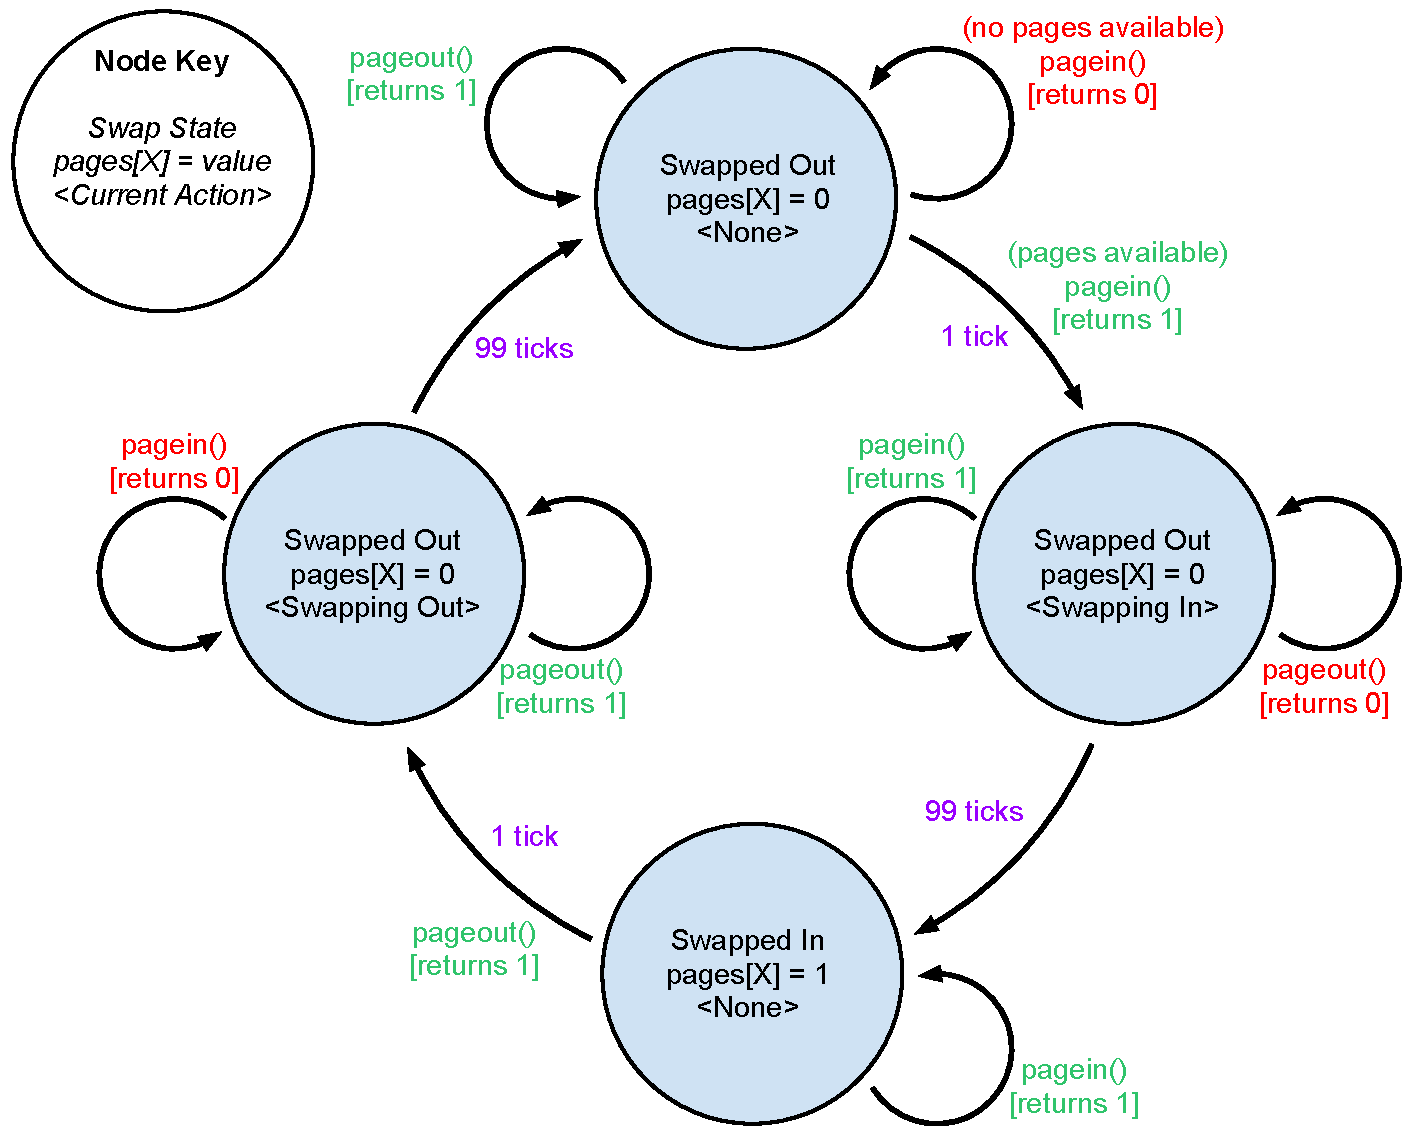
\includegraphics[width=0.75\textwidth]{simulator-PageState.pdf}
    \caption{Possible Page States and Transitions}
    \label{fig:pagestate}
  \end{center}
\end{figure}

Figure \ref{fig:pagestate} shows the possible states that a virtual
page can occupy, as well as the possible transitions between these
states. Note that the page map values alone do not define all possible
page states. We must also account for the possible operations
currently underway on a page to fully define its state. While the page
map for each process can be obtained from the \texttt{pageit} input
array of structs, there is no interface to directly reveal any
operations underway on a given page. If knowing whether or not a
paging operation is underway on a given page (and thus knowing the full
state of a page) is necessary for your \texttt{pageit} implementation, you
must maintain this data yourself.

\subsection {The Simulated Programs}

The simulator populates its 20 processes by randomly selecting processes
from a collection of 5 simulated ``programs''. Pseudo code for each of
the possible 5 programs is provided in Listings \ref{lst:pgm1} through
\ref{lst:pgm5}.

\lstinputlisting[
  caption={Test Program 1 - A loop with an inner branch},
  label=lst:pgm1
]{../pgm1.pseudo}

\lstinputlisting[
  caption={Test Program 2 - Single loop},
  label=lst:pgm2
]{../pgm2.pseudo}

\lstinputlisting[
  caption={Test Program 3 - Double Nested Loop},
  label=lst:pgm3
]{../pgm3.pseudo}

\lstinputlisting[
  caption={Test Program 4 - Linear},
  label=lst:pgm4
]{../pgm4.pseudo}

\lstinputlisting[
  caption={Test Program 5 - Probabilistic backward branch},
  label=lst:pgm5
]{../pgm5.pseudo}

This simple pseudo code notation shows you what will happen in each
process:
\begin{packed_item}
\item {\bf for X Y}: A ``for'' loop with between X and Y iterations
  (chosen randomly)
\item {\bf run Z}: Run Z (unspecified) instructions in sequence
\item {\bf if P}: Run next clause with probability P,
  run else clause (if any) with probability (1-P).
\item {\bf goto label}: Jump to ``label''
\end{packed_item}

As we discuss in the next section,
you may wish to use this knowledge about the possible programs to:
\begin{packed_enum}
\item Profile processes and know which kind of programs each is an
  instance of.
\item Use this knowledge to predict what pages a process will need
  in the future with rather high accuracy.
\end{packed_enum}

Note that while you know the structure of these programs, the programs
flow is still probabilistic in nature. Which branch a specific process
takes or how many loop iterations occur will be dependent upon the
random seed generated by the simulator. Thus, you may never be able to
perfectly predict the execution of a process, only the probabilistic
likelihood of a collection of possible execution paths.

\section{Some Implementation Ideas}

In general, your \texttt{pageit()} implementation will need to follow
the basic flow presented in Figure \ref{fig:pageit-reactive}. You will
probably spend most of your time deciding how to implement the ``Select
a Page to Evict'' element.

\begin{figure}[htbp]
  \begin{center}
    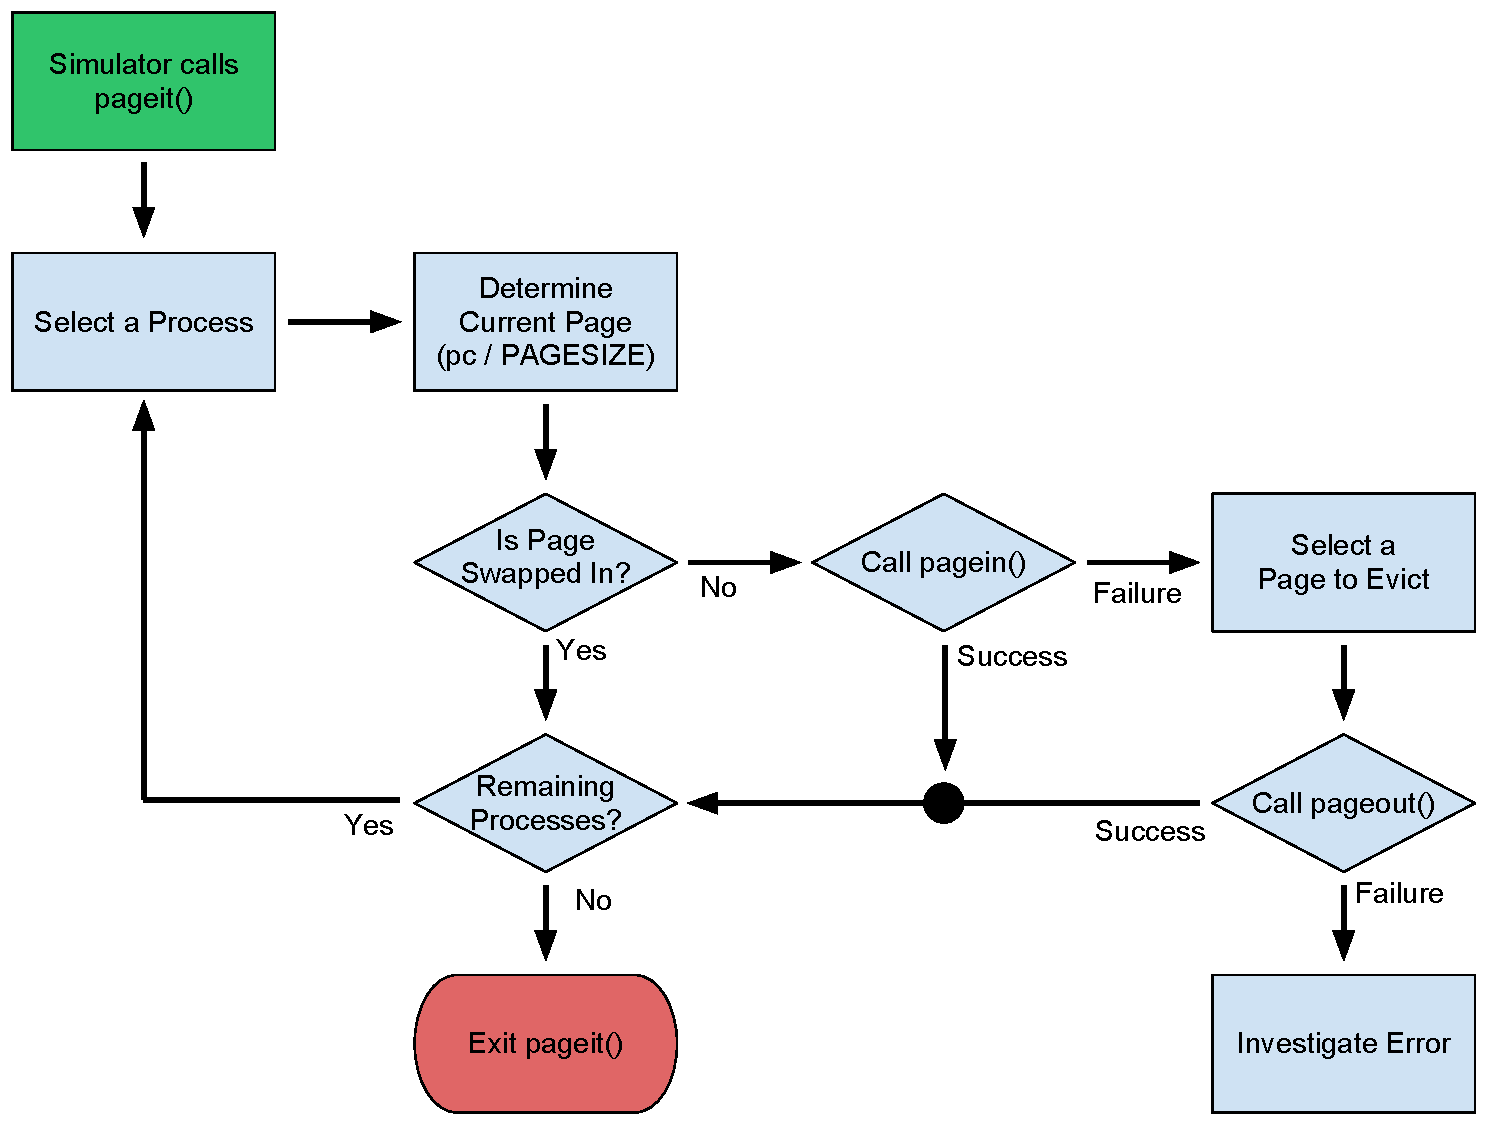
\includegraphics[width=0.8\textwidth]{pageit-Fig1.pdf}
    \caption{Basic Reactive \texttt{pageit()} Flow}
    \label{fig:pageit-reactive}
  \end{center}
\end{figure}

A basic ``one-process-at-a-time'' implementation is provided for
you. This implementation never actually ends up having to swap out any
pages. Since only one process is allocated pages at a time, no more than
20 pages are ever in use. When each process completes, it releases all
of its pages and the next process is allowed to allocate pages and
run. This is a very simple solution, and as you might expect, does not
provide very good performance. Still, it provides a simple starting
point that demonstrates the simulator API. See \texttt{pager-basic.c} for more
information.

To start, create some form of ``Least Recently Used'' (LRU) paging
algorithm. An LRU algorithm selects a page that has not been accessed
for some time when it must swap a page out to make room for a new
page to be swapped in. An LRU algorithm can either operate globally, or
with respect to a given process. In the latter case, you may wish to
pre-reserve a number of physical pages for each process and only allow
each process to compete for pages from this subset. An stub for
implementing your LRU version of \texttt{pageit()} has been created for
you in the \texttt{pager-lru.c} file. Note the use of static variables
in order to preserve local state between calls to \texttt{pageit()}.
Your LRU algorithm
should perform much better than the trivial solution discussed above,
but will still suffer from performance issues. We can do better.

To really do well on this assignment, you must create some form of
predictive paging algorithm. A predictive algorithm attempts to predict
what pages each process will require in the future and then swaps
these pages in before they are needed. Thus, when these pages are needed,
they are already swapped in and ready to go. The process need not
block to wait for the required pages to be swapped in, greatly
increasing performance. . Figure
\ref{fig:pageit-predictive} shows a modified version of the Figure
\ref{fig:pageit-reactive} flowchart for a predictive implementation of
\texttt{pageit}. As for the LRU implementation, a simple predictive stub
has been created for you in the \texttt{pager-predict.c} file.

\begin{figure}[htbp]
  \begin{center}
    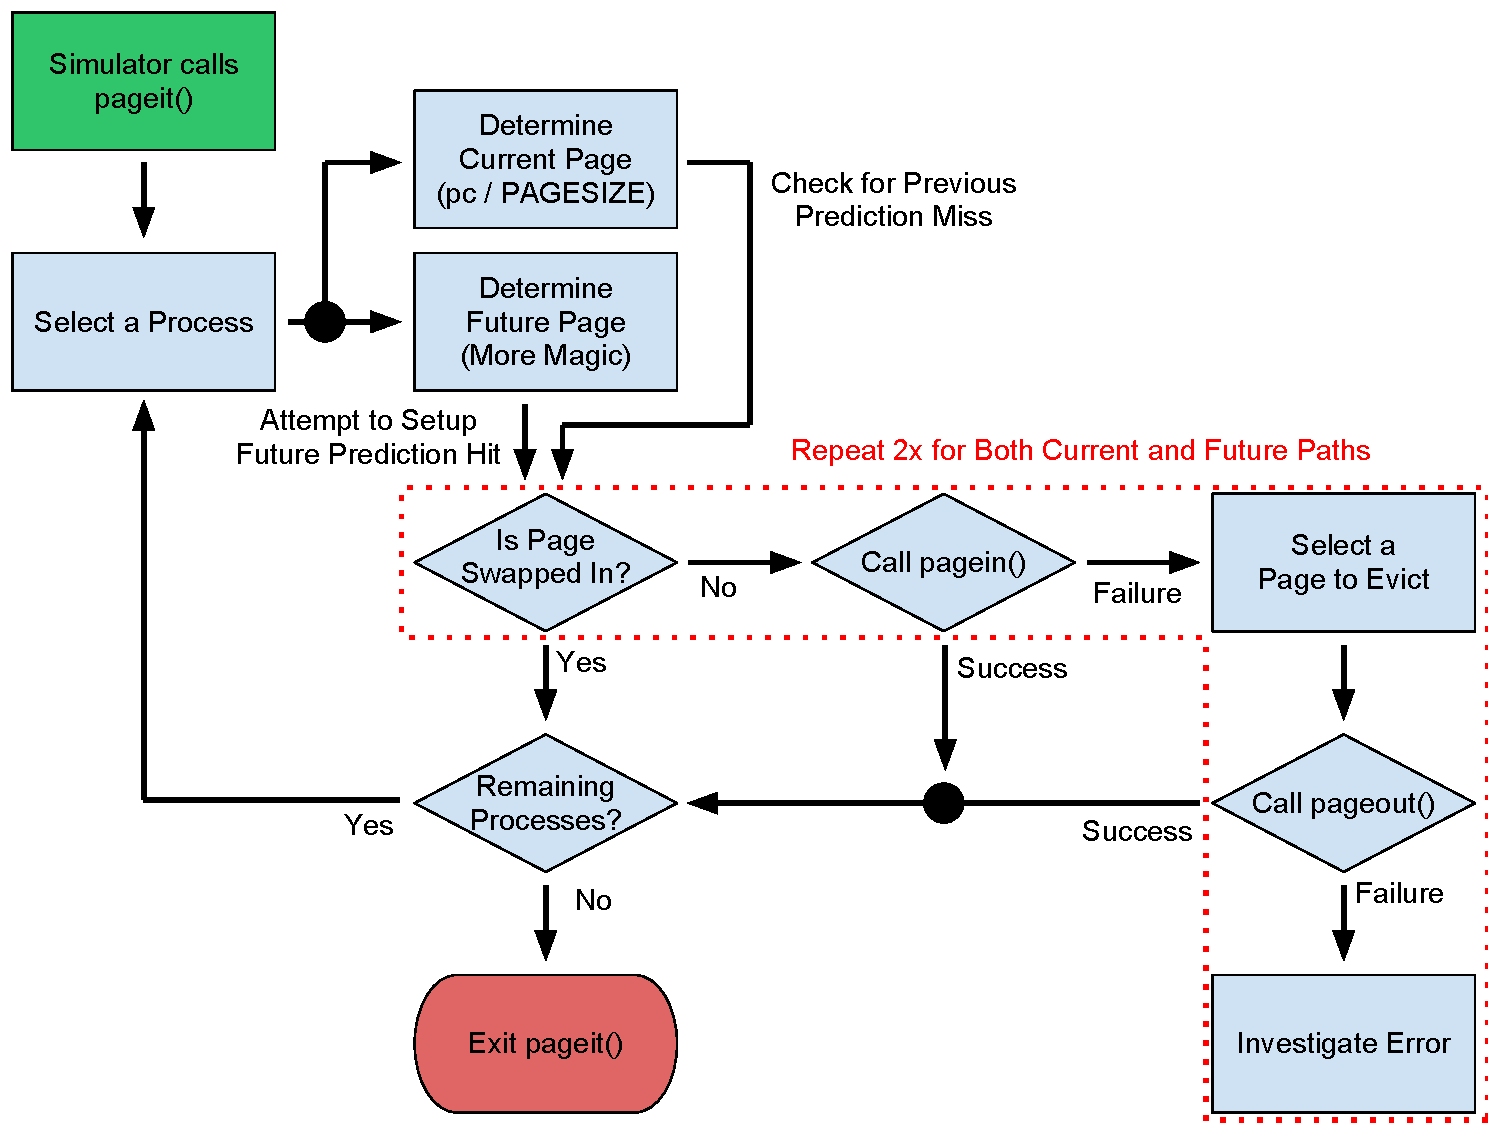
\includegraphics[width=0.8\textwidth]{pageit-Fig2.pdf}
    \caption{Basic Predictive \texttt{pageit()} Flow}
    \label{fig:pageit-predictive}
  \end{center}
\end{figure}

There are effectively two approaches to predictive algorithms. The
first approach is to leverage your knowledge of the possible program
types (see previous section). In this approach, one generally attempts
to heuristically determine which program each process is an instance of
by tracking the movement of the process's program counter (PC). Once each
process is classified, you can use further PC heuristics to determine where
in its execution the process is, and then implement a paging strategy
that attempts to swap in pages required by upcoming program actions
before they occur. Since the programs all have probabilistic elements,
this approach will never be perfect, but it can do very well.

The second approach to predictive algorithms is to ignore the
knowledge you have been given regarding the various program
types. Instead, you might track each process's program counter to try
to detect various common patterns (loops, jumps to specific locations,
etc). If you detect a pattern, you assume that the pattern will continue to
repeat and attempt to swap in the necessary pages touched during the
execution of the pattern before the process needs them.
Working set algorithms are a subset of this approach.

Note that in any predictive operation, you ideally wish to stay
100-200 ticks ahead of the execution of each process. This is the
necessary predictive lead time in which you must make paging decisions
in order to insure that the necessary pages are available when the
process reaches them and that no blocking time is required. As Figure
\ref{fig:pageit-predictive} shows, in addition to swapping in pages
predicatively, you must still handle the case where your prediction has
failed and are thus forced to reactively swap in the necessary
page. This is referred to as a predictive miss. A good predictive
algorithm will minimize misses, but still must handle them when they
occur. In other words, you can not assume that your predictions will
always works and that every currently needed page is already
available. Doing so will most likely lead to deadlock.

There are a number of additional predictive notions that might prove
useful involving state-space analysis \cite{wiki-statespace}, Markov
chains \cite{wiki-markov},  and similar techniques.
We will leave such solutions to the student to investigate if she
wishes. Please see the references section for additional information
and ideas.

\section{What's Included}

We provide some code to help get you started. Feel free to use it as a
jumping off point (appropriately cited).

\begin{packed_enum}
\item {\bf Makefile} A GNU Make makefile to build all the code listed
  here.
\item {\bf README} As the title so eloquently instructs: read it.
\item {\bf simulator.c} The core simulator source code. For reference
  only.
\item {\bf simulator.h} The simulator header file including the simulator
  API.
\item {\bf programs.c} Struct representing simulated programs for use
  by simulator. For reference and use by simulator code only.
\item {\bf pager-basic.c} A basic paging implementation that only runs
  one process at a time.
\item {\bf pager-lru.c} A stub for your LRU paging implementation.
\item {\bf pager-predict.c} A stub for your predictive paging implementation.
\item {\bf api-test.c} A pageit implementation that detects and prints
  simulator state changes. May be useful if you want to confirm the
  behavior of the simulator API. Builds to \texttt{test-api}.
\item {\bf test-*} Executable test programs. Runs the simulator using
  your pager-*.c strategy. Built using \texttt{Makefile}. The simulator
  provides a lot of tools to help you analyze your program.
  Run \texttt{./test-* -help} for information on available options. It
  also responds to various signals by printing the current page table
  and process execution state to the screen (try \texttt{ctrl-c} while
  simulator is executing).
\item {\bf test-api} An API test program. See \texttt{api-test.c}.
\item {\bf see.R} An R script for displaying a visualization of the
  process run/block activity in a simulation.
  You must first run \texttt{./test-* -csv} to
  generate the necessary trace files. To run visualization, lunch R in
  windowed graphics mode (in Linux: \texttt{R -g Tk \&} at the command
  prompt) from the directory containing the trace
  files (or use \texttt{setwd} to set your working directory to the directory
  containing the trace files). Then run \texttt{source(``see.r'')} at the R
  command prompt to lunch the visualization.
\end{packed_enum}

\section{What You Must Provide}

When you submit your assignment, you must provide the following as a
single archive file:
\begin{packed_enum}
\item A copy of your LRU paging implementation
\item A copy of your best predictive paging implementation
\item A makefile that builds any necessary code
\item A README explaining how to build and run your code
\end{packed_enum}

\section{Grading}

40\% of you grade will be based on the performance of the
best pager implementation that you provide. The following simulation
scores will earn the corresponding number of points:
\begin{packed_item}
\item Code does not compile without errors : 0 Points
\item $score >= 1.28$ : 5 Points
\item $0.64 <= score < 1.28$ : 10 Points
\item $0.32 <= score < 0.64$ : 15 Points (Basic LRU implementation)
\item $0.16 <= score < 0.32$ : 20 Points
\item $0.08 <= score < 0.16$ : 25 Points
\item $0.04 <= score < 0.08$ : 30 Points
\item $0.02 <= score < 0.04$ : 35 Points
\item $0.01 <= score < 0.02$ : 40 Points (Good predictive implementation)
\item $0.005 <= score < 0.01$ : 40 Points + 5 Points EC
\item $score < 0.005$ : 40 Points + 10 Points EC (Excellent predictive implementation)
\end{packed_item}

During your grading session, we will run your code using several
random seeds and will take the average of these runs as your
score. Thus, if your program's performance varies widely from
run-to-run, you may get bitten in the grading session. In the words of
Client Eastwood, ``Do I feel lucky?''.

If your code generates warnings when building under gcc on the VM
using \texttt{-Wall} and \texttt{-Wextra} you will be penalized 1
point per warning. In addition, to receive full credit your submission must:
\begin{packed_item}
\item Meet all requirements elicited in this document
\item Code must adhere to good coding practices.
\item Code must be submitted to Moodle prior to due date.
\end{packed_item}

The other 60\% of your grade will be determined via your grading
interview where you will be expected to explain your work and answer
questions regarding it and any concepts related to this assignment.

\section{Obtaining Code}
The starting code for this assignment is available on the Moodle and
on github. If you would like practice using a version control system,
consider forking the code from github. Using the github code is not
a requirement, but it will help to insure that you stay up to date
with any updates or changes to the supplied codebase. It is also
good practice for the kind of development one might expect to do in
a professional environment. And since your github code can be easily
shared, it can be a good way to show off your coding skills to
potential employers and other programmers.

Github code may be forked from the project page here:\\
\url{https://github.com/asayler/CU-CS3753-2012-PA4}.

\section{Resources}
Refer to your textbook and class notes on the Moodle for an overview
of OS paging policies and implementations.

If you require a good C language reference, consult K\&R\cite{K+R}.

The Internet\cite{tubes} is also a good resource for finding
information related to solving this assignment.

The most recent version of the assignment from which this assignment
was adopted is available at \cite{couch-a5}.

You may wish to consult the man pages for the following items, as they
will be useful and/or required to complete this assignment. Note that
the first argument to the ``man'' command is the chapter, insuring
that you access the appropriate version of each man page. See
\texttt{man man} for more information.

\begin{packed_item}
\item \texttt{man 1 make}
\end{packed_item}

\begin{thebibliography}{3}

\bibitem{couch-a5} Couch, Alva.
  \newblock \emph{Comp111 - A5}.
  \newblock Tufts University: Fall 2011.
  \newblock \url{http://www.cs.tufts.edu/comp/111/assignments/a5.html}.

\bibitem{K+R} Kernighan, Brian and Dennis, Ritchie.
  \newblock \emph{The C Programming Language}.
  \newblock Second Edition: 2009.
  \newblock Prentice Hall: New Jersey.

\bibitem{tubes} Stevens, Ted.
  \newblock \emph{Speech on Net Neutrality Bill}.
  \newblock 2006.
  \newblock \url{http://youtu.be/f99PcP0aFNE}.

\bibitem{wiki-statespace} Wikipedia.
  \newblock ``State space (dynamical system)''.
  \newblock Wikipedia, The Free Encyclopedia. 2012.
  \newblock
  \url{http://en.wikipedia.org/w/index.php?title=State_space_(dynamical_system)&oldid=478401148}.
  \newblock Online; accessed 12-April-2012.

\bibitem{wiki-markov} Wikipedia.
  \newblock ``Markov chain''.
  \newblock Wikipedia, The Free Encyclopedia. 2012.
  \newblock
  \url{http://en.wikipedia.org/w/index.php?title=Markov_chain&oldid=486910550}.
  \newblock Online; accessed 12-April-2012.

\end{thebibliography}

\end{document}  
